% Appendix A: development-suite analyses (moved out of the main text).
% Labels app:dev / app:rq1 / app:rq2 / app:rq3 / app:rq4 / app:efficiency.
\section{Development-Suite Analyses}
\setcounter{table}{0}
\label{app:dev}
\label{sec:results}

\emph{In one sentence:} this appendix reports the design-phase analyses in full --- data quality, the four research questions, and the budget-efficiency simulations --- with the caveat that all of them are exploratory (Section~\ref{sec:stats}) and were later re-evaluated on the held-out suite (Section~\ref{sec:heldout}).

These analyses established the conditions, the regime strata, and the allocation rules on the development suite (six systems, 90 questions, per-model coverage 12 to 90), and all of them are exploratory in the sense of Section~\ref{sec:stats}. The three follow-up controls (greedy paraphrases, the MMLU-Pro probe, and chain-of-thought answering) are reported in \ref{app:greedypara}--\ref{app:cot} as descriptive robustness checks.

\subsection{Overview and data quality}
\label{app:overview}
\label{sec:overview}

\emph{In one sentence:} answer extraction succeeds on 94.7--100 percent of calls; complete-matrix exclusions follow provider rate limits on a fixed question order, and two sensitivity analyses bound their effect.

Table~\ref{tab:models} summarizes the ten evaluated systems across the two suites. Answer extraction succeeds on between 94.7\% and 100\% of calls across models; cells whose first decode fails to parse were re-drawn under the identical configuration until extraction succeeded, subject to provider quota. Qwen3.8-Max reached a complete sixteen-call matrix on all ninety questions; Qwen3.8-Omni reached it on seventy-one of the ninety, and the remaining four models on 12 to 40 questions each, bounded by provider rate limits and free-tier quotas. All within-model comparisons are paired and unaffected by coverage, and pooled analyses use the intersection of completed questions, stated explicitly wherever pooled numbers appear.

\begin{table}[htbp]
\centering
\small
\caption{Main results on the development suite. Accuracy (\%) under budget-matched conditions: greedy single call at $\tau{=}0$, single-sample expectation S1 (mean over the six canonical draws at $\tau{=}0.7$), six-vote self-consistency (SC-6), six-paraphrase ensemble (PE-6), three-paraphrase two-sample hybrid (HB-6), and the twelve-vote combined ensemble (COMB-12). $\Delta$SC and $\Delta$PE are the gains of SC-6 and PE-6 over the S1 baseline in points.}
\label{tab:main}
\scriptsize
\begin{tabular*}{\columnwidth}{@{\extracolsep{\fill}} l c c c c c c c c c}
\toprule
Model & $n$ & Greedy & S1 & SC-6 & PE-6 & HB-6 & COMB-12 & $\Delta$SC & $\Delta$PE \\
\midrule
Qwen3.8-Max & 90 & 93.3 & 93.3 & 93.3 & 93.3 & 92.2 & 93.3 & +0.0 & +0.0 \\
Qwen3.8-Omni & 71 & 93.0 & 93.9 & 93.0 & 93.0 & 91.5 & 93.0 & -0.9 & -0.9 \\
Agnes3.0-Flash & 33 & 78.8 & 89.4 & 90.9 & 90.9 & 90.9 & 90.9 & +1.5 & +1.5 \\
Agnes2.5-Flash & 40 & 90.0 & 94.2 & 95.0 & 92.5 & 92.5 & 95.0 & +0.8 & -1.7 \\
GPT-6-Luna & 15 & 80.0 & 76.7 & 73.3 & 86.7 & 86.7 & 86.7 & -3.3 & +10.0 \\
Gemini3.8-Flash & 12 & 91.7 & 86.1 & 83.3 & 91.7 & 91.7 & 91.7 & -2.8 & +5.6 \\
\bottomrule
\end{tabular*}
\end{table}

The sensitivity analysis in Table~\ref{tab:models} addresses the residual exclusions from two directions. Under a lenient aggregation rule that admits any question with at least four parsed votes per source, the ordering of conditions is preserved for every model: Agnes3.0-Flash moves from 78.8\% greedy to 88.1\% under SC-6 and 92.3\% under PE-6 on the extended set, and the flagship accuracies shift by at most one question. Comparing excluded with included questions on greedy accuracy shows that the excluded sets are not systematically easier: for Qwen3.8-Omni the excluded questions are nine points \emph{harder} (84.2\% versus 93.0\%), for Agnes2.5-Flash they are thirty points harder (60.0\% versus 90.0\%), while for GPT-6-Luna and Gemini3.8-Flash the few excluded questions happened to be answered correctly. The exclusions follow provider rate limits on a fixed question order rather than any adaptive choice, and both checks indicate that the complete-matrix requirement does not manufacture the effects we report.

\subsection{RQ1: Accuracy under budget-matched ensembling}
\label{app:rq1}
\label{sec:rq1}

\emph{In one sentence:} on the development suite no systematic gain for either source over S1 is detected; the largest movements sit where the modal answer is wrong, and the greedy reference diverges from S1 on specific endpoints.

Table~\ref{tab:main} reports accuracy for the five aggregation conditions together with the two single-call baselines, and Figure~\ref{fig:conditions} visualizes the four models with at least twenty complete questions. Because the ensembles spend stochastic calls, the single-sample expectation S1 is the primary $k{=}1$ baseline, and the $\Delta$ columns of Table~\ref{tab:main} express both ensemble gains relative to it. Three patterns dominate. First, the two Qwen flagships are at or near ceiling on five of six benchmarks, and for them the pure ensembles reproduce both baselines exactly: SC-6, PE-6, and COMB-12 all return 93.3\% for Qwen3.8-Max and 93.0\% for Qwen3.8-Omni, identical to greedy and S1. The aggregation strategies are not failing; they are vacuous, because the answer distribution they aggregate contains a single value, a point that Section~\ref{app:rq4} quantifies. Second, measured against S1, no systematic gain for either diversity source is detected in this data: pooled over the four well-covered models (112 model-question pairs on 28 common questions), SC-6 gains $+0.9$ points and PE-6 loses $0.9$ points, with the combined ensemble exactly matching S1; the largest per-model gain over S1 is $+1.5$ points (Agnes3.0-Flash, both sources). Third, the gains that do exist are concentrated where the modal answer is wrong, and are exploratory at these sample sizes: PE-6 lifts GPT-6-Luna by $+10.0$ points over S1 ($n=15$, CI $[0.0, +22.2]$) and Gemini3.8-Flash by $+5.6$ ($n=12$, CI $[0.0, +13.9]$), while SC-6 \emph{loses} $3.3$ and $2.8$ points on the same two models (both intervals spanning zero). The wrong-mode condition itself holds clearly only on their LogiQA subsets (five and three questions), so we read the direction as consistent with the plurality-vote signature of Section~\ref{sec:condorcet} rather than as an established per-model effect.

\begin{figure}[htbp]
\centering
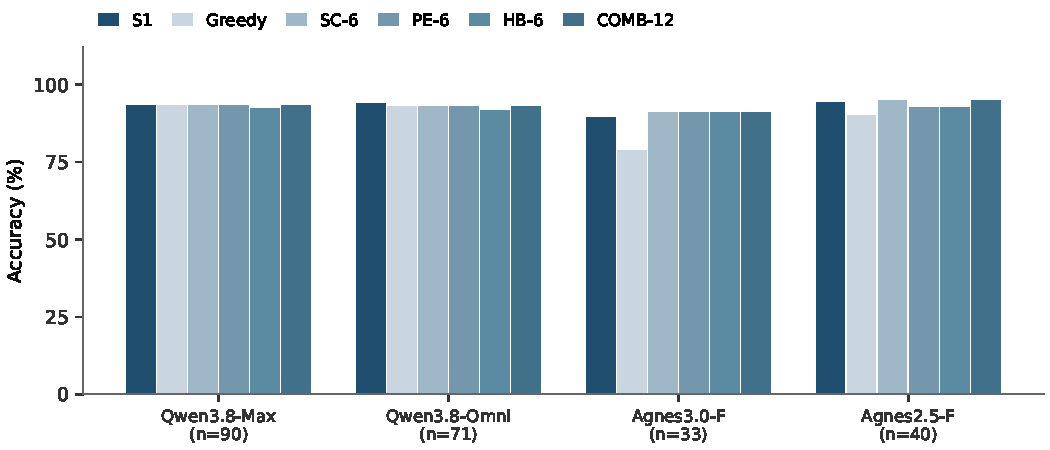
\includegraphics[width=\columnwidth]{figures/conditions.pdf}
\caption{Accuracy of the single-sample baseline S1, the greedy reference, and the four aggregation conditions for the four models with at least twenty complete question matrices. The two Qwen flagships show identical accuracy across conditions, which reflects answer degeneracy rather than agreement between strategies; the models where the modal answer is wrong (GPT-6-Luna, Gemini3.8-Flash) show the two diversity sources pulling in opposite directions. Exact values are given in Table~\ref{tab:main}.}
\label{fig:conditions}
\end{figure}

A separate result concerns the greedy reference itself: greedy decoding at $\tau = 0$ is not an unbiased stand-in for a single stochastic draw. Pooled over the same 112 pairs, S1 reaches 96.4\% against 92.0\% for greedy, a $+4.5$ point gap whose question-level cluster-bootstrap interval, $[+0.9, +8.8]$, excludes zero. The gap is model dependent in both direction and mechanism. For the two Agnes models, greedy sits $10.6$ and $4.2$ points below S1; auditing the discordant questions shows one clear truncation artifact (a greedy chain-of-thought that hit the token cap, after which the parser extracted an intermediate number), two cases of mode locking where the greedy answer differed from every one of the six sampled answers, and remaining cases where greedy picks a minority answer. For GPT-6-Luna and Gemini3.8-Flash the sign reverses ($-3.3$ and $-5.6$ points), and for these models the greedy answer always coincided with the modal sampled answer on our data. Neither baseline subsumes the other, which is why Table~\ref{tab:main} reports both; but because the ensembles aggregate stochastic calls, S1 is the fair comparison, and gains measured against greedy conflate the ensembling effect with the greedy-versus-sampled gap. For a practitioner who currently deploys only greedy decoding, the most direct consequence is a decoding recommendation rather than an ensembling one: on the affected Agnes endpoints, replacing the greedy call with a single stochastic draw at the same budget already recovers four to eleven points in our data. The raw outputs of every audited discordant question --- the truncation artifact, the mode-locking cases, and the minority picks --- are included in the released supplementary material (greedy-bias audit) so that each mechanism can be inspected directly. Section~\ref{sec:heldout} adds the decisive qualification: on the held-out suite, the gap reappears on only one of four endpoints, so the divergence documented here is a property of specific model--endpoint configurations, not a general property of greedy decoding.

Two further observations complete the accuracy picture. The hybrid allocation is a hedge rather than a dominant strategy: it matches the better pure strategy when one source fails, as for GPT-6-Luna where HB-6 and PE-6 both reach 86.7\% while SC-6 falls to 73.3\%, but it never exceeds the better pure strategy on any model, and it trails it by exactly one question on Qwen3.8-Max (92.2 versus 93.3), Qwen3.8-Omni (91.5 versus 93.0), and Agnes2.5-Flash (92.5 versus 95.0). The twelve-vote combined ensemble likewise does not dominate the six-vote conditions: pooled it exactly matches S1 at 96.4\% against 97.3\% for SC-6, because for three of the four pooled models the paraphrase votes it adds are individually no better than a single canonical draw and dilute the majority. Doubling the budget therefore buys no guarantee; the quality of the marginal vote, not the count, governs the outcome.

On the central question, whether one diversity source buys more accuracy per call than the other, no difference is detected in this data against either baseline. Against S1, the pooled SC-6 advantage over PE-6 is $1.8$ points --- two (model, question) pairs out of 112, both resolved in favor of SC-6 --- with a question-level cluster-bootstrap 95\% interval of $[0.0, +5.4]$ (the 90\% interval that the TOST procedure operates on is $[0.0, +3.6]$), and the per-model intervals for the gain over S1 all include zero (Table~\ref{tab:tests}); no per-model McNemar test on the SC-6-versus-PE-6 discordances approaches significance (all $p \ge 0.5$), and the smallest McNemar $p$ anywhere in the table is $0.125$ (SC-6 versus greedy on Agnes3.0-Flash), which does not survive any multiple-comparison correction. We emphasize what this does and does not establish. The TOST procedure at equivalence bounds of $\pm 3$ points does not conclude equivalence for the pooled difference, and the bound itself is coarse at these sample sizes: $\pm 3$ points is 2.7 questions at $n = 90$ and fewer than one question on the smallest sets, so a single flipped question can move the verdict. At these sample sizes the study is powered to detect only large differences; a genuine advantage of either source of up to several points could go unnoticed. The two strategies are therefore not interchangeable in principle, and for two reasons the data show they are not interchangeable in practice either: they disagree on individual questions at measurable rates (Section~\ref{app:rq2}), and their agreement signals catch different errors (Section~\ref{app:rq3}).

\begin{table}[htbp]
\centering
\footnotesize
\caption{Paired comparisons between conditions on the development suite: discordant counts ($b$: first condition right, second wrong; $c$: the reverse), exact McNemar $p$, accuracy difference with 95\% question-resampled bootstrap CI, and the TOST verdict at $\pm 3$ point equivalence bounds. ``no'' means equivalence is not established at this sample size, not that a difference was found.}
\label{tab:tests}
\scriptsize
\begin{tabular*}{\columnwidth}{@{\extracolsep{\fill}} l c l c c c c c c}
\toprule
Model & $n$ & Comparison & $b$ & $c$ & McNemar $p$ & Diff. & 95\% CI & TOST $\pm$3 \\
\midrule
Qwen3.8-Max & 90 & SC-6 $-$ S1 & -- & -- & -- & +0.0 & [0.0,0.0] & -- \\
 &  & PE-6 $-$ S1 & -- & -- & -- & +0.0 & [0.0,0.0] & -- \\
 &  & SC-6 $-$ Greedy & 0 & 0 & 1.000 & +0.0 & [0.0,0.0] & -- \\
 &  & SC-6 $-$ PE-6 & 0 & 0 & 1.000 & +0.0 & [0.0,0.0] & yes \\
\addlinespace
Qwen3.8-Omni & 71 & SC-6 $-$ S1 & -- & -- & -- & -0.9 & [-3.3,1.2] & -- \\
 &  & PE-6 $-$ S1 & -- & -- & -- & -0.9 & [-4.0,1.6] & -- \\
 &  & SC-6 $-$ Greedy & 1 & 1 & 1.000 & +0.0 & [-4.2,4.2] & -- \\
 &  & SC-6 $-$ PE-6 & 1 & 1 & 1.000 & +0.0 & [-4.2,4.2] & yes \\
\addlinespace
Agnes3.0-Flash & 33 & SC-6 $-$ S1 & -- & -- & -- & +1.5 & [-2.5,6.1] & -- \\
 &  & PE-6 $-$ S1 & -- & -- & -- & +1.5 & [-2.5,6.1] & -- \\
 &  & SC-6 $-$ Greedy & 4 & 0 & 0.125 & +12.1 & [3.0,24.2] & -- \\
 &  & SC-6 $-$ PE-6 & 0 & 0 & 1.000 & +0.0 & [0.0,0.0] & yes \\
\addlinespace
Agnes2.5-Flash & 40 & SC-6 $-$ S1 & -- & -- & -- & +0.8 & [0.0,2.5] & -- \\
 &  & PE-6 $-$ S1 & -- & -- & -- & -1.7 & [-5.0,0.0] & -- \\
 &  & SC-6 $-$ Greedy & 2 & 0 & 0.500 & +5.0 & [0.0,12.5] & -- \\
 &  & SC-6 $-$ PE-6 & 1 & 0 & 1.000 & +2.5 & [0.0,7.5] & no \\
\addlinespace
GPT-6-Luna & 15 & SC-6 $-$ S1 & -- & -- & -- & -3.3 & [-12.2,4.4] & -- \\
 &  & PE-6 $-$ S1 & -- & -- & -- & +10.0 & [0.0,22.2] & -- \\
 &  & SC-6 $-$ Greedy & 0 & 1 & 1.000 & -6.7 & [-20.0,0.0] & -- \\
 &  & SC-6 $-$ PE-6 & 0 & 2 & 0.500 & -13.3 & [-33.3,0.0] & no \\
\addlinespace
Gemini3.8-Flash & 12 & SC-6 $-$ S1 & -- & -- & -- & -2.8 & [-12.5,4.2] & -- \\
 &  & PE-6 $-$ S1 & -- & -- & -- & +5.6 & [0.0,13.9] & -- \\
 &  & SC-6 $-$ Greedy & 0 & 1 & 1.000 & -8.3 & [-25.0,0.0] & -- \\
 &  & SC-6 $-$ PE-6 & 0 & 1 & 1.000 & -8.3 & [-25.0,0.0] & no \\
\bottomrule
\end{tabular*}
\end{table}

The comparison is also matched in tokens, not only in calls. Averaged per call, canonical-sample and paraphrase calls cost within one to five percent of each other for every model (for example 223 versus 219 tokens for Qwen3.8-Max and 505 versus 528 for GPT-6-Luna), because validated paraphrases change the surface form but not the length of the task: the mean character-length ratio between paraphrase and original stems is 1.06 for the Qwen models and 1.13 to 1.14 for the API-served models. Budgets matched in calls are therefore approximately matched in cost for this suite.

\subsection{RQ2: Paraphrase fragility}
\label{app:rq2}
\label{sec:rq2}

\emph{In one sentence:} fragility is negligible in the degenerate regime and substantial in the high-entropy regime, and on this suite flips were an entirely stem-locus phenomenon --- a locus split the held-out suite later corrected (Section~\ref{sec:heldoutfragility}).

Fragility, the fraction of questions where paraphrasing alone flips the majority answer, is negligible in the degenerate regime and substantial in the high-entropy regime. Qwen3.8-Max shows fragility on 1.1\% of questions and Qwen3.8-Omni on 4.2\%, concentrated almost entirely in LogiQA, where the respective per-dataset fragility rates are 6.7\% and 21.4\%. The models with high answer entropy on logical reasoning show more: GPT-6-Luna flips on 13.3\% of its questions overall and on 40\% of its LogiQA questions, and Gemini3.8-Flash on 8.3\% overall and 33.3\% of LogiQA. Agnes3.0-Flash, whose gains come with fully consistent votes across both sources, shows zero fragility.

Stratifying by paraphrase locus, which the design fixes in advance, showed flips on this suite to be an entirely stem-locus phenomenon: across all six models, no question flipped under instruction paraphrasing (zero of 52 pooled instruction-locus pairs), while 3.3\% of pooled stem-locus pairs flipped, rising to 28.6\% and 20\% for GPT-6-Luna and Gemini3.8-Flash respectively. The two loci differ by construction in how much of the prompt they vary, so the asymmetry should be read as a property of the perturbation family rather than of the models: instruction rewordings touch only the answer-format scaffolding, while stem rewordings touch the problem content itself. For evaluation practice, the practical consequence is that a single-prompt score on a hard benchmark understates the instability of the measured system by an amount that stem fragility makes visible. The held-out suite, however, shows that the sharper half of this reading was a property of the question draw rather than a structural law: on the fresh questions, instruction-locus flips do occur (9.6\% pooled against 17.4\% for stem-locus), concentrated exactly where the handcrafted instruction variants differ in elicitation quality, on SAT-Math (Section~\ref{sec:heldoutfragility}). Instruction-level paraphrase ensembling therefore probes a weaker axis of variation than stem-level paraphrasing on average, but not a structurally safe one.

Fragility is not random noise; it tracks the same model-task cells that carry answer entropy and ensembling gains, which supports reading it as an observable symptom of unstable knowledge rather than as a formatting artifact. It is also not an artifact of loose paraphrases: recomputing the statistic with only the paraphrases whose fresh embedding similarity exceeds the stricter 0.80 threshold, requiring at least four such paraphrases per question, leaves the rates essentially unchanged or higher for every model (GPT-6-Luna 33.3\% on six qualifying questions versus 13.3\% overall; Gemini3.8-Flash 25.0\% versus 8.3\%; Qwen3.8-Omni 4.8\% versus 4.2\%), so if anything the tighter paraphrases flip more. \ref{app:greedypara} returns to fragility with a decoding-noise-free variant computed from greedy paraphrase decodes, and Section~\ref{sec:heldoutfragility} recomputes the fragility statistics on the held-out suite, where they carry larger denominators and a corrected locus split.

\subsection{RQ3: Consistency as an error signal}
\label{app:rq3}
\label{sec:rq3}

\emph{In one sentence:} on the development suite, models with genuine entropy show informative agreement scores and the stronger source differs across models --- readings that rest on one to three errors and are reported as descriptive only; the held-out recomputation at adequate error counts overturned the sharpest of them (Section~\ref{sec:heldouterror}).

Table~\ref{tab:uncert} evaluates agreement scores as unsupervised detectors of ensemble errors, and Figure~\ref{fig:auroc} visualizes AUROC. Models with fewer than five ensemble errors are marked with a dagger and reported descriptively only; at one to three errors, AUROC values are dominated by individual questions and their confidence intervals would span most of the unit interval. The held-out suite supplies the error counts this analysis needs --- twelve to twenty-one ensemble errors per fully covered model --- and Section~\ref{sec:heldouterror} reports the recomputation; the readings below are the development suite's, and two of them did not survive the recomputation. The pattern follows the regime structure. For the Qwen flagships, where almost every question is degenerate, sample agreement carries almost no signal (AUROC 0.58 for Qwen3.8-Max, 95\% CI $[0.50, 0.78]$) because the score is constant at one for nearly all questions, right or wrong; the degenerate stratum contributes errors that are invisible to any agreement-based detector by construction, and five of Qwen3.8-Max's six errors are missed by both signals. Qwen3.8-Omni retains moderate signal (0.79). In the models with genuine entropy the scores become informative and the stronger source differs across models: for Agnes3.0-Flash, sample agreement reads as highly discriminative (0.96, CI $[0.89, 1.00]$) while paraphrase agreement reads as weak (0.60); for GPT-6-Luna paraphrase agreement is the stronger signal (0.92 against 0.58) and for Gemini3.8-Flash both signals separate its single error perfectly. Agnes2.5-Flash, whose answers are mostly degenerate, shows a reversed sample-agreement ranking that we read as noise at its two-error rate. The Agnes3.0-Flash reading is the one the held-out suite overturned: at eighteen errors the two signals are comparable there (0.80 against 0.81), so the development-suite contrast should be read as an artifact of the three-error denominator, exactly what the five-error rule of Section~\ref{sec:method} was designed to flag.

\begin{table}[htbp]
\centering
\footnotesize
\caption{Uncertainty estimation on the development suite. Error rate of the COMB-12 reference; AUROC of reversed agreement scores for predicting ensemble errors (95\% bootstrap CI where the model has at least five errors); and the area under the risk-coverage curve (AURC; lower is better), computed by accepting questions in decreasing order of confidence with ties broken uniformly at random and averaged over 1{,}000 permutations, so a random ranking yields AURC equal to the error-rate column. Both is the sum of the two disagreement scores (AUROC only). $^\dagger$Fewer than five errors: descriptive only. Dashes indicate constant scores or zero errors.}
\label{tab:uncert}
\footnotesize
\begin{tabular*}{\columnwidth}{@{\extracolsep{\fill}} l c c c c c c}
\toprule
 & & \multicolumn{3}{c}{AUROC} & \multicolumn{2}{c}{AURC$^{\ddagger}$} \\
\cmidrule(lr){3-5}\cmidrule(lr){6-7}
Model & Err. & $c_S$ & $c_P$ & Both & $c_S$ & $c_P$ \\
\midrule
Qwen3.8-Max & 6.7 & 0.583 & 0.576 & 0.578 & 0.057 & 0.058 \\
Qwen3.8-Omni & 7.0 & 0.788 & 0.779 & 0.780 & 0.031 & 0.032 \\
Agnes3.0-Flash$^\dagger$ & 9.1 & 0.961 & 0.600 & 0.922 & 0.009 & 0.073 \\
Agnes2.5-Flash$^\dagger$ & 5.0 & 0.487 & 0.704 & 0.704 & 0.051 & 0.029 \\
GPT-6-Luna$^\dagger$ & 13.3 & 0.577 & 0.923 & 0.769 & 0.105 & 0.024 \\
Gemini3.8-Flash$^\dagger$ & 8.3 & 0.955 & 0.955 & 1.000 & 0.011 & 0.011 \\
\bottomrule
\end{tabular*}
\end{table}

\begin{figure}[htbp]
\centering
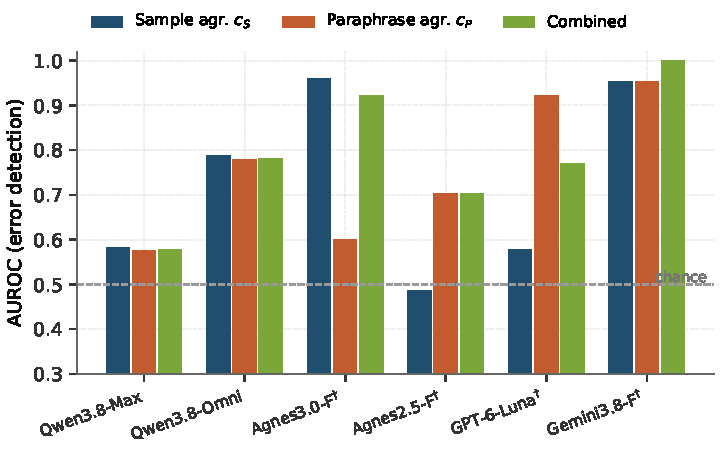
\includegraphics[width=0.8\columnwidth]{figures/auroc.pdf}
\caption{AUROC of reversed agreement scores for detecting ensemble errors. The dashed line marks chance. Signal strength follows the entropy regime, and the stronger source differs across models. $^\dagger$Models with fewer than five errors, reported descriptively.}
\label{fig:auroc}
\end{figure}

The risk-coverage analysis in Table~\ref{tab:uncert} quantifies the selective-prediction value of each signal, with ties in the confidence score resolved by uniformly random tie-breaking (Section~\ref{sec:method}), so each AURC is directly comparable with the model's overall error rate, which is the AURC of a random ranking. Sample agreement attains an AURC of 0.031 for Qwen3.8-Omni against an error rate of 7.0\%, and 0.009 for Agnes3.0-Flash against 9.1\%; paraphrase agreement attains 0.032 and 0.073 on the same models, so the AURC ordering tracks the AUROC ordering, and each value sits below its model's error rate as expected when the ranking carries signal. For Qwen3.8-Max, whose signals are uninformative, AURC stays at 0.057 against a 6.7\% error rate, close to the random baseline as expected. Pooled over the four well-covered models, sample agreement reaches an AUROC of 0.74 (cluster-bootstrap 95\% CI $[0.71, 0.75]$) against 0.60 $[0.46, 0.73]$ for paraphrase agreement, an interval that overlaps chance: pooled across models with opposite signal strengths, the paraphrase signal averages out.

The two agreement scores therefore measure different failure modes, but the evidence for complementarity is about coverage, not about a superior combined detector. Among the ensemble errors of the models with informative signals, the flagged sets overlap only partially: for Agnes3.0-Flash, sample agreement flags all three errors while paraphrase agreement flags one, two of them only through sample agreement; for GPT-6-Luna, paraphrase agreement flags both errors and sample agreement only one; for Qwen3.8-Omni the two signals flag the same three of five errors. Accordingly, the combined Both score exceeds the best single signal only for Gemini3.8-Flash, ties it for Agnes3.0-Flash (0.92 against 0.96 for sample agreement alone, i.e., slightly below), and falls between the two singles elsewhere; pooled it reaches 0.73 against 0.74 for sample agreement alone. A deployment that can afford both probes obtains partially disjoint evidence, and neither signal subsumes the other. On this suite the simple sum of the two disagreement scores does not dominate the best single signal; the held-out suite, at adequate error counts, reversed that reading (Section~\ref{sec:heldouterror}), so we treat the combination question as open rather than settled against the sum, with a learned or calibrated combination remaining the natural next step. We also note the structural caveat of Section~\ref{sec:method}: on questions where all twelve votes coincide, the reference answer equals that unanimous vote by construction, so detectors that read unanimity are correct by definition on the degenerate stratum; the informative content of Table~\ref{tab:uncert} lies in the non-degenerate stratum, which the flagged-error analysis above reflects.

\subsection{RQ4: The regime structure}
\label{app:rq4}
\label{sec:rq4}

\emph{In one sentence:} disagreement predicts the fragility of the greedy reference rather than the value of ensembling; the sign of the ensemble gain is set by whether the modal answer is correct, and high-dissent cells are small and descriptive.

Table~\ref{tab:regime} reports per model and dataset the greedy accuracy, the single-sample expectation, the combined-ensemble accuracy, the gain of the latter over the former, the mean modal vote share, and the mean dissent share (one minus the modal share), and Figure~\ref{fig:regime} plots the ensemble gain over S1 against the dissent share for every model-dataset cell. The scatter shows the dependency that anchors the whole study. Disagreement predicts the fragility of the greedy reference rather than the value of ensembling: across the pooled (model, question) pairs of the four well-covered models, the Spearman rank correlation between the dissent share and the gap $\mathrm{S1} - \mathrm{greedy}$ is $+0.80$, meaning that greedy decoding departs furthest from the sampled consensus exactly where the votes disagree, while the correlation between dissent and the COMB-12 gain over S1 is only $+0.17$: relative to a single stochastic draw, ensembling neither gains nor loses much on average, it only converts an uncertain single draw into the modal answer. Both correlations must be read with their tie structure in mind: 104 of the 112 pooled pairs are unanimous, on them the gap is nonzero exactly once and the COMB-12 answer never differs from S1, so the rank ordering is determined by the eight non-unanimous pairs, within which the gap correlation is $+0.57$; using the absolute gap instead of the signed gap leaves the pooled value unchanged at $+0.80$. Because the combined share and the combined ensemble draw on the same twelve votes, we also recompute the ensemble-gain correlations with strictly disjoint votes: the sample-side dissent share against the PE-6 gain over S1 gives $-0.20$, and the paraphrase-side dissent share against the SC-6 gain over S1 gives $+0.54$, both resting on the same eight informative pairs and read as descriptive. The stratified view makes the structure explicit: the pooled pairs split 104 unanimous, five with a strong majority (share at least two thirds), and three with a weak or no majority. In the unanimous stratum the sampled conditions all sit at 98.1\% (greedy at 97.1\%), and the combined ensemble returns exactly the S1 answer on every one of the 104 unanimous pairs. In the five strong-majority pairs, S1 is 76.7\% and the six-vote ensembles 80.0\%. In the three weak-majority pairs, S1 is 72.2\%, SC-6 reaches 100\%, PE-6 falls to 33.3\%, and the combined ensemble 66.7\%; with three pairs these numbers are descriptive, but they display the full plurality-vote signature of Section~\ref{sec:condorcet}: aggregation pays where the mode is right and is destructive where it is wrong.

\begin{table}[htbp]
\centering
\footnotesize
\caption{Regime map by model and dataset: greedy accuracy, single-sample expectation S1, COMB-12 accuracy, the COMB-12 gain over S1 ($\Delta_C$), the mean modal vote share over the twelve stochastic votes, and the mean dissent share (one minus the modal share, in percent).}
\label{tab:regime}
\scriptsize
\begin{tabular*}{\columnwidth}{@{\extracolsep{\fill}} l l c c c c c c c}
\toprule
Model & Dataset & $n$ & Greedy & S1 & COMB & $\Delta_C$ & Share & Diss.\% \\
\midrule
Qwen3.8-Max & GSM8K & 15 & 100.0 & 100.0 & 100.0 & +0.0 & 100.0 & 0.0 \\
Qwen3.8-Max & SAT-Math & 15 & 100.0 & 100.0 & 100.0 & +0.0 & 100.0 & 0.0 \\
Qwen3.8-Max & PIQA & 15 & 100.0 & 100.0 & 100.0 & +0.0 & 98.9 & 1.1 \\
Qwen3.8-Max & TruthfulQA & 15 & 100.0 & 100.0 & 100.0 & +0.0 & 100.0 & 0.0 \\
Qwen3.8-Max & LSAT-LR & 15 & 100.0 & 100.0 & 100.0 & +0.0 & 100.0 & 0.0 \\
Qwen3.8-Max & LogiQA & 15 & 60.0 & 60.0 & 60.0 & +0.0 & 97.2 & 2.8 \\
\midrule
Qwen3.8-Omni & GSM8K & 15 & 100.0 & 100.0 & 100.0 & +0.0 & 100.0 & 0.0 \\
Qwen3.8-Omni & SAT-Math & 1 & 100.0 & 100.0 & 100.0 & +0.0 & 91.7 & 8.3 \\
Qwen3.8-Omni & PIQA & 11 & 100.0 & 100.0 & 100.0 & +0.0 & 100.0 & 0.0 \\
Qwen3.8-Omni & TruthfulQA & 15 & 93.3 & 96.7 & 93.3 & -3.3 & 96.1 & 3.9 \\
Qwen3.8-Omni & LSAT-LR & 15 & 100.0 & 98.9 & 100.0 & +1.1 & 99.4 & 0.6 \\
Qwen3.8-Omni & LogiQA & 14 & 71.4 & 73.8 & 71.4 & -2.4 & 89.3 & 10.7 \\
\midrule
Agnes3.0-Flash & GSM8K & 7 & 85.7 & 97.6 & 100.0 & +2.4 & 94.0 & 6.0 \\
Agnes3.0-Flash & SAT-Math & 2 & 100.0 & 100.0 & 100.0 & +0.0 & 95.8 & 4.2 \\
Agnes3.0-Flash & PIQA & 5 & 100.0 & 100.0 & 100.0 & +0.0 & 100.0 & 0.0 \\
Agnes3.0-Flash & TruthfulQA & 5 & 100.0 & 100.0 & 100.0 & +0.0 & 100.0 & 0.0 \\
Agnes3.0-Flash & LSAT-LR & 6 & 83.3 & 88.9 & 83.3 & -5.6 & 95.8 & 4.2 \\
Agnes3.0-Flash & LogiQA & 8 & 37.5 & 66.7 & 75.0 & +8.3 & 84.4 & 15.6 \\
\midrule
Agnes2.5-Flash & GSM8K & 7 & 85.7 & 100.0 & 100.0 & +0.0 & 98.8 & 1.2 \\
Agnes2.5-Flash & SAT-Math & 11 & 100.0 & 100.0 & 100.0 & +0.0 & 99.2 & 0.8 \\
Agnes2.5-Flash & PIQA & 7 & 85.7 & 85.7 & 85.7 & +0.0 & 98.8 & 1.2 \\
Agnes2.5-Flash & TruthfulQA & 4 & 100.0 & 100.0 & 100.0 & +0.0 & 100.0 & 0.0 \\
Agnes2.5-Flash & LSAT-LR & 6 & 83.3 & 83.3 & 83.3 & +0.0 & 100.0 & 0.0 \\
Agnes2.5-Flash & LogiQA & 5 & 80.0 & 93.3 & 100.0 & +6.7 & 90.0 & 10.0 \\
\midrule
GPT-6-Luna & GSM8K & 1 & 100.0 & 100.0 & 100.0 & +0.0 & 100.0 & 0.0 \\
GPT-6-Luna & SAT-Math & 5 & 80.0 & 80.0 & 80.0 & +0.0 & 96.7 & 3.3 \\
GPT-6-Luna & PIQA & 2 & 100.0 & 100.0 & 100.0 & +0.0 & 100.0 & 0.0 \\
GPT-6-Luna & TruthfulQA & 2 & 100.0 & 100.0 & 100.0 & +0.0 & 100.0 & 0.0 \\
GPT-6-Luna & LogiQA & 5 & 60.0 & 50.0 & 80.0 & +30.0 & 73.3 & 26.7 \\
\midrule
Gemini3.8-Flash & GSM8K & 1 & 100.0 & 100.0 & 100.0 & +0.0 & 100.0 & 0.0 \\
Gemini3.8-Flash & SAT-Math & 4 & 100.0 & 100.0 & 100.0 & +0.0 & 93.8 & 6.2 \\
Gemini3.8-Flash & PIQA & 2 & 100.0 & 100.0 & 100.0 & +0.0 & 100.0 & 0.0 \\
Gemini3.8-Flash & TruthfulQA & 2 & 100.0 & 100.0 & 100.0 & +0.0 & 100.0 & 0.0 \\
Gemini3.8-Flash & LogiQA & 3 & 66.7 & 44.4 & 66.7 & +22.2 & 66.7 & 33.3 \\
\bottomrule
\end{tabular*}
\end{table}

\begin{figure}[htbp]
\centering
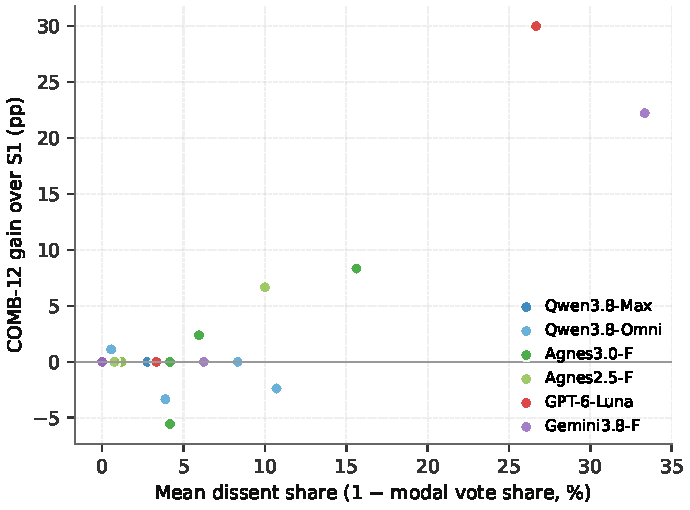
\includegraphics[width=0.75\columnwidth]{figures/regime.pdf}
\caption{Combined-ensemble gain over the single-sample baseline S1 against the mean dissent share (one minus the modal vote share) for every model-dataset cell. Every zero-dissent cell sits exactly at S1. The largest gains sit at the highest dissent: LogiQA under GPT-6-Luna ($+30.0$ points, $n=5$) and LogiQA under Gemini3.8-Flash ($+22.2$, $n=3$), where the sample-side modal answer is wrong while the paraphrase side carries the correct majority into the combined vote. Losses appear at moderate dissent (up to $-5.6$ for LSAT-LR under Agnes3.0-Flash), so the sign of the gain depends on whether the modal answer is correct, not on the amount of disagreement; high-dissent cells contain five questions or fewer, and the pattern is descriptive.}
\label{fig:regime}
\end{figure}

Within the high-dissent region, the two largest gains of the study sit on the two cells with the most dissent, and both are carried by the paraphrase side. Under GPT-6-Luna on LogiQA ($n=5$), the single-sample expectation is 50\%, the six-sample majority drops to 40\% because the modal sampled answer is wrong, while the paraphrase majority rises to 80\% and takes the combined ensemble with it, a $+30.0$ point gain over S1. The LogiQA cell of Gemini3.8-Flash ($n=3$) shows the same signature at smaller scale: S1 is 44.4\%, the sample majority 33.3\%, the paraphrase majority 66.7\%, and the combined ensemble follows it for a $+22.2$ point gain. The plurality-vote model of Section~\ref{sec:condorcet} summarizes the pattern: disagreement is a necessary condition for aggregation to matter at all, but the sign of the gain is determined by which side holds the correct majority, which the dissent share alone does not measure. Both cells are small --- five and three questions --- so we read them as the clearest descriptive illustrations of the mechanism rather than as precise estimates of its size.

The budget curves in Figure~\ref{fig:budget} complete the picture, with the single-sample baseline S1 at $k=1$ and the greedy level marked as a dotted line; panel headers state how many percentage points one question contributes, since a single flipped question moves accuracy by 1.1 to 3.0 points at these sample sizes. For the flagships the curves are flat at the greedy level within one question at every budget, with the one-question deviations reflecting individual tie-breaks rather than trends: Qwen3.8-Max dips one question under PE at $k \in \{2,4\}$, and Qwen3.8-Omni wiggles one question above greedy under SC-4. For Agnes3.0-Flash, the paraphrase ensemble reaches its full 90.9\% already at $k=2$ while the sample majority needs $k=4$ to catch up, the two curves crossing rather than one leading throughout. For Agnes2.5-Flash the ordering is the reverse and persists: sample voting climbs to 95.0\% by $k=6$ while paraphrase voting plateaus at 92.5\%. The practical reading is that the choice between the two sources matters less than the choice of whether to aggregate at all, which the disagreement regime determines, and that neither source dominates the other in budget profile across models.

\begin{figure}[htbp]
\centering
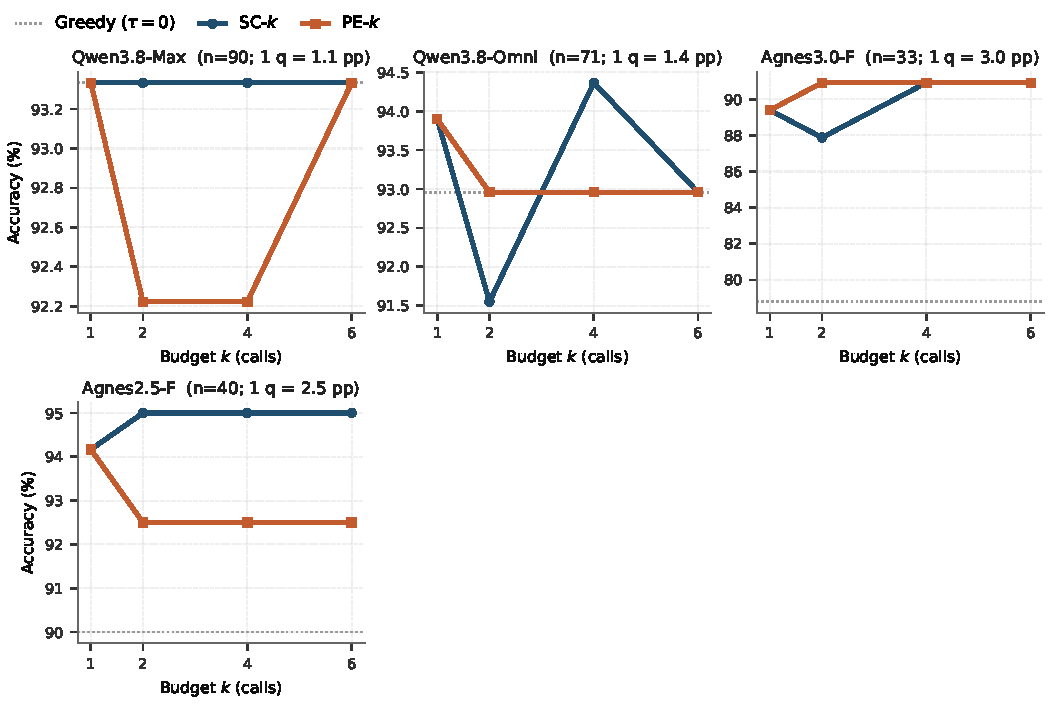
\includegraphics[width=\columnwidth]{figures/budget.pdf}
\caption{Accuracy against call budget $k$ for self-consistency (SC-$k$) and paraphrase ensembling (PE-$k$), with the single-sample baseline S1 at $k=1$ and the greedy accuracy as a dotted line. Panel headers give each model's question count and the accuracy value of one question. Flat curves indicate the degenerate regime; rising or crossing curves indicate cells where aggregation changes answers.}
\label{fig:budget}
\end{figure}

\subsection{Budget efficiency: early stopping and adaptive allocation}
\label{app:efficiency}
\label{sec:efficiency}

\emph{In one sentence:} on the development suite the unanimity rule preserves SC-6 accuracy at two to three calls, and the adaptive rule matches the best fixed strategy on four of six models at 68--78 percent of the budget --- a consistency check, not a validation; the fresh-question transfer test is Section~\ref{sec:heldoutrule}.

The regime structure implies that most of a fixed budget is spent confirming answers that additional calls cannot change. Two simulated policies quantify the waste; both are replays of our own data rather than new methods, and both descend from existing work on sample-adaptive stopping: the sequential unanimity rule is a special case of the early-stopping self-consistency line \citep{aggarwal2023lets,li2024escape}, and we read our simulation as a reproduction of that line's finding in the direct-answering, near-degenerate regime rather than as a novel contribution. The unanimity rule draws canonical samples until the first $k$ at which all drawn samples agree, answers with that unanimous vote, and otherwise falls back to the six-sample majority. The adaptive allocation rule of Section~\ref{sec:discussion} probes each question with two canonical samples and two paraphrases, then routes the remaining budget to paraphrases, resampling, or a split according to which side shows diversity. Table~\ref{tab:efficiency} reports both policies against the fixed conditions, with the probe's calls charged to the adaptive rule; its mean budget runs 4.1 to 4.7 calls, 68 to 78 percent of the six-call budget.

\begin{table}[htbp]
\centering
\footnotesize
\caption{Budget efficiency on the development suite. Accuracy (\%) of the fixed conditions against the sequential unanimity rule (ES, with mean budget $\bar{k}$) and the adaptive allocation rule (Ada, with mean budget and its share of the six-call budget), both simulated on the collected call matrices.}
\label{tab:efficiency}
\scriptsize
\begin{tabular*}{\columnwidth}{@{\extracolsep{\fill}} l c c c c c c c c c}
\toprule
Model & S1 & SC-6 & PE-6 & ES acc & ES $\bar{k}$ & Ada acc & Ada $\bar{k}$ & Budget & COMB-12 \\
\midrule
Qwen3.8-Max & 93.3 & 93.3 & 93.3 & 93.3 & 2.0 & 93.3 & 4.1 & 68\% & 93.3 \\
Qwen3.8-Omni & 93.9 & 93.0 & 93.0 & 93.0 & 2.2 & 91.5 & 4.3 & 71\% & 93.0 \\
Agnes3.0-Flash & 89.4 & 90.9 & 90.9 & 90.9 & 2.5 & 90.9 & 4.6 & 77\% & 90.9 \\
Agnes2.5-Flash & 94.2 & 95.0 & 92.5 & 95.0 & 2.1 & 92.5 & 4.2 & 70\% & 95.0 \\
GPT-6-Luna & 76.7 & 73.3 & 86.7 & 80.0 & 2.0 & 86.7 & 4.5 & 76\% & 86.7 \\
Gemini3.8-Flash & 86.1 & 83.3 & 91.7 & 83.3 & 2.7 & 91.7 & 4.7 & 78\% & 91.7 \\
\bottomrule
\end{tabular*}
\end{table}

The unanimity rule preserves SC-6 accuracy within one question for every model at a mean budget of 2.0 to 2.7 calls, because degenerate questions announce themselves after two or three unanimous draws. The adaptive rule matches the best fixed six-call strategy on four of the six models and trails it by exactly one question on the remaining two, Qwen3.8-Omni (91.5 against 93.0) and Agnes2.5-Flash (92.5 against 95.0), while spending a mean of 4.1 to 4.7 calls, 68 to 78 percent of the six-call budget; it never exceeds the best fixed strategy on any model, and the one-question deficits are exactly the questions whose diversity the two-call probe did not reveal. The comparison against the fixed paraphrase ensemble is the sharpest way to state what the rule adds: the adaptive rule's accuracy equals PE-6's on five of the six models and sits one question below it on Qwen3.8-Omni, so on this data its realized allocation reproduces PE-6 at 68 to 78 percent of its calls. Its increment is the call saving, not accuracy --- the accuracy advantage exists only against a misallocated fixed budget such as SC-6 on GPT-6-Luna --- and on Agnes2.5-Flash it forgoes the one-question edge that fixed SC-6 holds over PE-6 there. A rule worth its added complexity over always running PE-6 must therefore be justified on fresh questions and harder distributions, where the probe's routing can matter in both directions. Because the rule was designed and evaluated on the same collected matrices, this simulation is a consistency check on the rule, not a validation of it; Section~\ref{sec:heldoutrule} performs the fresh-question transfer test. The savings are conservative estimates: the simulation commits to a fixed routing rule after the probe rather than continuing to monitor agreement as later calls arrive, and it charges the full probe even on questions where one call would have sufficed. Both simulations are exact replays of the released call matrices, so they can be re-derived from the logs.
